%-------------------------------------------------------------------------------
% 请勿删除本注释
% Free Response Question 1
%
% 指引:
% 如在小问之前有通用问题描述,请放置于此
%-------------------------------------------------------------------------------
\begin{figure}[H]
\centering
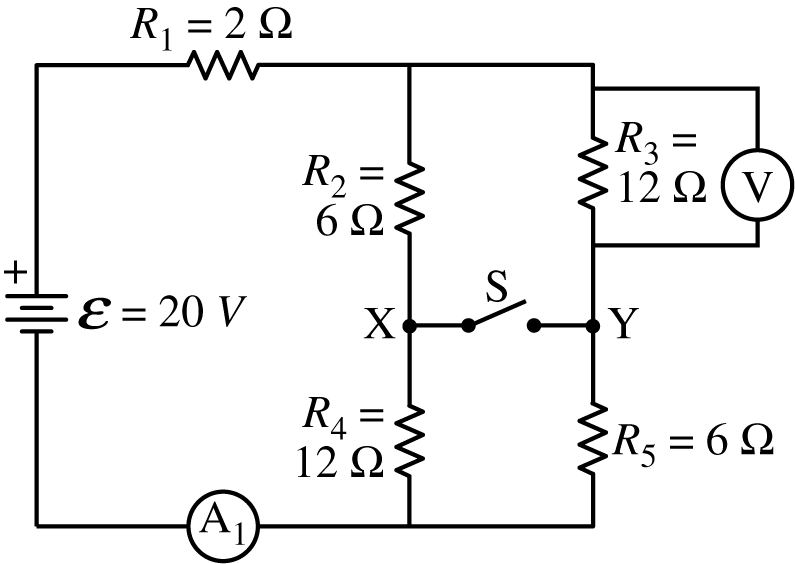
\includegraphics[scale=0.3]{images/img-018-034.png}
\end{figure}



\question
A circuit is created with an ideal battery and five resistors with the values shown in the figure above. An open switch is shown that can connect points X and Y. A voltmeter V and an ammeter $\mathrm{A_{1}}$ are also shown in the figure. % 请删除并替换本行,与上一行 \question 之间不要留空行

\begin{parts}

%-------------------------------------------------------------------------------
% 请勿删除本注释
% Part (a)
%
% 指引:
% 如在小问之前有通用问题描述,请放置于此
%-------------------------------------------------------------------------------

\part
The switch is in the open position. % 请删除并替换本行,与上一行 \part 之间不要留空行
\begin{subparts}
\subpart Calculate the current measured by the ammeter $\mathrm{A}_{1}$. 
\subpart Calculate the potential difference measured by the voltmeter $\mathrm{V}$.
\end{subparts}

%-------------------------------------------------------------------------------
% 请勿删除本注释
% Part (b)
%
% 指引:
% 如在小问之前有通用问题描述,请放置于此
%-------------------------------------------------------------------------------

\part
The switch is now moved to the closed position. % 请删除并替换本行,与上一行 \part 之间不要留空行
\begin{subparts}
\subpart Calculate the current measured by the ammeter $\mathrm{A}_{1}$.
\subpart Calculate the potential difference measured by the voltmeter $\mathrm{V}$.
\end{subparts}

%-------------------------------------------------------------------------------
% 请勿删除本注释
% Part (c)
%
% 指引:
% 如在小问之前有通用问题描述,请放置于此
%-------------------------------------------------------------------------------

\part
A student wants to determine if there is a current in the closed switch. The switch is now replaced with ammeter $\mathrm{A}_{2}$ between points $\mathrm{X}$ and $\mathrm{Y}$. The ammeter acts as a closed switch and can measure the current, if any, between the two points. % 请删除并替换本行,与上一行 \part 之间不要留空行

\begin{figure}[H]
\centering
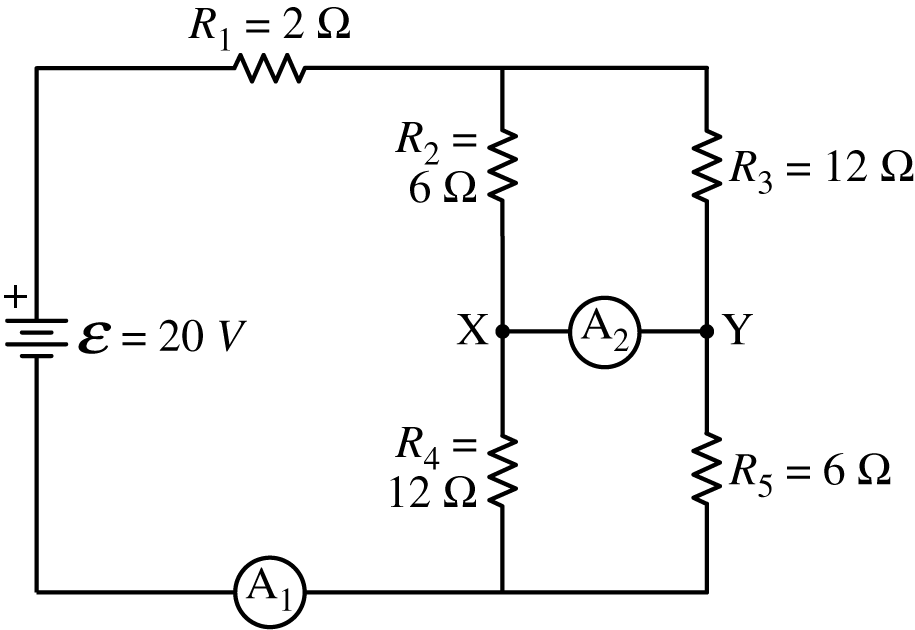
\includegraphics[scale=0.3]{images/img-019-035.png}
\end{figure}

\begin{subparts}
\subpart Calculate the current measured by ammeter $\mathrm{A}_{2}$.
\subpart Indicate the direction of the current, if any, through the ammeter $\mathrm{A}_{2}$.
\end{subparts}

\underline{\qquad}Left \qquad  \underline{\qquad}Right \qquad  \underline{\qquad}Undefined, because the current is zero

%-------------------------------------------------------------------------------
% 请勿删除本注释
% Part (d)
%
% 指引:
% 如在小问之前有通用问题描述,请放置于此
%-------------------------------------------------------------------------------
\begin{figure}[H]
\centering
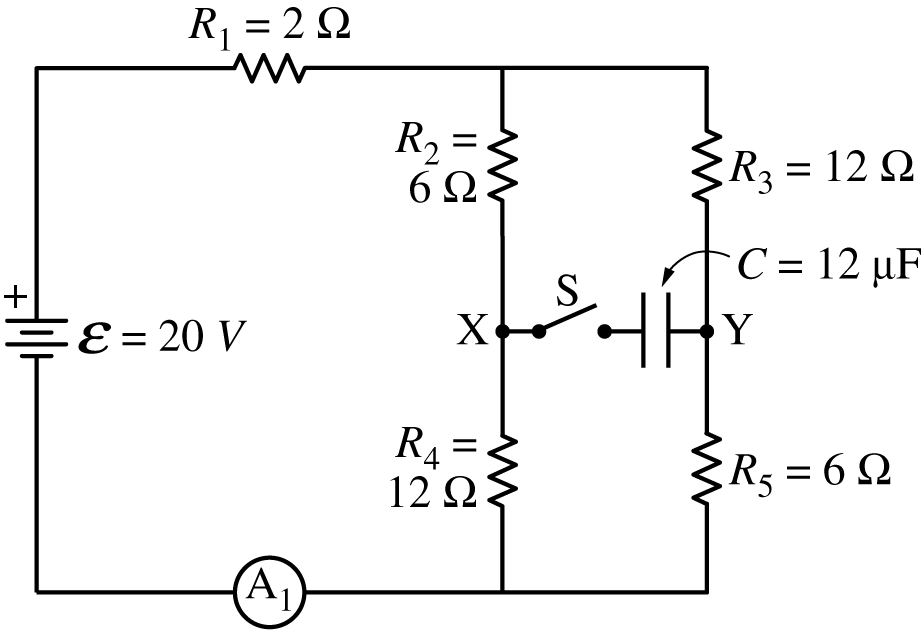
\includegraphics[scale=0.3]{images/img-020-036.png}
\end{figure}

\part
The ammeter $\mathrm{A}_{2}$ is replaced with switch $\mathrm{S}$ and capacitor $C=12 \mu \mathrm{F}$, as shown in the figure above. Switch $S$ is closed. % 请删除并替换本行,与上一行 \part 之间不要留空行
\begin{subparts}
\subpart Calculate the charge stored on the positive plate of capacitor $C$ a long time after switch $S$ is closed.
\subpart Which point, $\mathrm{X}$ or $\mathrm{Y}$, is at a higher electric potential?
\end{subparts}

\underline{\qquad}X  \qquad \underline{\qquad}Y

Justify your answer.


\end{parts}
